\documentclass[a4paper, 12pt, headsepline]{scrartcl}

\usepackage[a4paper, left=3cm, right=2cm, top=2.5cm, bottom=2.5cm]{geometry}
%encoding
\usepackage[utf8]{inputenc}
\usepackage[T1]{fontenc}

%German-specific commands
\usepackage[ngerman]{babel}

%Hyphenation rules
\usepackage{hyphenat}

\usepackage{setspace}
\usepackage{parskip}

%Für quots
\usepackage[autostyle=true, german=quotes]{csquotes}

%Für Abbildungen
\usepackage{graphicx}

\usepackage{ragged2e}
\usepackage[format=plain,
      justification=RaggedRight,
      singlelinecheck=false]
     {caption}
  
% Inhaltsverwaltung wird eingefügt
\usepackage[style=authortitle, citestyle=authoryear]{biblatex}

%Klickbares Inhaltsverzeichnis
\usepackage[hidelinks]{hyperref}
\hypersetup{
	allcolors=black,
	linktoc=all,
}

%Um auf ein Bild innerhalb eines Textes referieren zu können
\usepackage[ngerman]{cleveref}

\addbibresource{references.bib}

\onehalfspacing

\begin{document}

\begin{titlepage}
\begin{center}


\includegraphics[width=5cm,right]{Assets/TH-Wildau-Logo_rgb}

\vspace{1cm}

\textbf{\huge
Bachelorarbeit
}
\vspace{1.3cm}
		
zur Erlangung des akademischen Grades \\
Bachelor

\vspace{2cm}

\textbf{ \large
Technische Hochschule Wildau \\
Fachbereich Wirtschaft, Informatik, Recht \\
Studiengang Wirtschaftsinformatik (B. Sc.)
}

\vspace{1.4cm}

\textbf{Thema (Deutsch)} \\
Die Umstellung von einer monolithischen Architektur auf eine Microservice-Architektur \\
am Beispiel von PluraPolit

\vspace{.5cm}

\textbf{Thema (Englisch)} \\
The conversion from a monolithic architecture to a microservice architecture \\
using the example of the startup PluraPolit

\vspace{1.5cm}

		\end{center}
\begin{description}
	\item [Autor] Edgar Muss
	\item [Matrikelnummer] 50033021
	\item [Seminargruppe] I1/16
	\item [Betreuer] Prof. Dr. Christian Müller
	\item [Zweitgutachter] Prof. Dr. Mike Steglich
	\item [Eingereicht am] 14.07.2020
\end{description}
\end{titlepage}

\newpage
\pagenumbering{Roman}

\section*{Abstract}

\newpage

\tableofcontents

\newpage
\pagenumbering{arabic}
\setcounter{page}{1}
\section{Einleitung}

Für ein junges Unternehmen, im Bereich der digitalen Produktentwicklung, ist es wichtig, schnell Ideen umzusetzen und erstes Feedback zu erhalten. Dies helft bei der Bestätigung von Annahmen und bei der Beschaffung von Investoren.

Diese schnelle Softwareentwicklung führt jedoch zu einigen Abstrichen hinsichtlich der Qualität. So wird zu Beginn oftmals auf einen automatischen Prozess zur Bereitstellung der Applikation verzichtet und leicht umsetzbare Lösungen vor langfristigen bevorzugt. Auch hinsichtlich der Auswahl der Architektur wird anfängliche Performance als oberstes Auswahlkriterium bestimmt. Endet der Weg für ein Start-up nicht nach wenigen Monaten, dann müssen die ursprünglichen Entscheidungen hinterfragt werden.

Genau an diesem Punkt ist das junge Unternehmen PluraPolit, welches sich erst Mitte letzten Jahres gegründet hat und innerhalb von wenigen Monaten ein fertiges Produkt entwickelte. PluraPolit hat sich zur Aufgabe gestellt eine Bildungsplattform für Jung- und Erstwähler zu Entwicklern und bei der Meinungsbildung zu unterstützen. Gefördert wird das Projekt von der Zentrale für politische Bildung und ist politisch unabhängig. Des Weiteren handelt es sich bei PluraPolit um ein gemeinnütziges Unternehmen, welches keine Absicht verfolgt, Gewinne auszuzahlen. Ich bin seit Anfang Januar an diesem Projekt beteiligt und begleite es seitdem als Frontendentwickler. Gemeinsam mit einem der drei Gründer sind wir zu zweit die technische Abteilung des Unternehmens und kümmern uns um die Weiterentwicklung der Plattform.

Die Inhalte der Plattform werden von den zwei anderen Gründern gepflegt und eingeholt. Es handelt sich dabei um neun verschiedene Tonaufnahmen zu einer Frage. Die Audioaufzeichnung kommen ausschließlich von Politikern und beziehen sich auf eine aktuelle politische Fragestellung. So gibt es zum Beispiel das Thema: Sollte der öffentlich-rechtliche Rundfunk abgeschafft werden? Die jeweiligen Politikerinnen und Politiker werden direkt zu einem Statement angefragt, welches anschließend ohne inhaltliche Veränderung auf die Webseite geladen wird. Angefragt werden immer alle Parteien, die im Bundestag vertreten sind. Neben Fragen, die ausschließlich von Politikern diskutiert werden, kommen gleichermaßen Themen auf die Plattform, die von den jeweiligen Expertinnen und Experten beantwortet werden. So gibt es bei der oben genannten Fragestellung auch eine Äußerung des Vertreters der Landesrundfunkanstalten ARD. Im Gegensatz zu anderen Anbieter für Nachrichten rund um Politik, stellt PluraPolit ausschließlich Sprachnachrichten auf die Plattform, die von jeweiligen Expertinnen und Experten kommen. Es wurde sich exklusiv für das Medium Tonaufnahme entscheiden, um eine junge Zielgruppe anzusprechen und die einzelnen Beiträge wie einen Podcast hören zu können.

\subsection{Problemstellung}

Umgesetzt wurde die Plattform in Ruby on Rails\footnote{
Ruby on Rails ist ein quellenoffenes Webframework, welches für die Programmiersprache Ruby entwickelt wurde \parencites{ruby_org}[vgl.][S. 24]{sieben_wochen}.
} im Backend und React.js\footnotemark im Frontend. Dabei liefert das Backend auf Anfrage Inhalte an das Frontend und kümmert sich um die Speicherung von Daten. Das Frontend im Gegensatz fordert beim Laden der Webseite alle genötigten Informationen an und stellt sie anschließend dar. Trotz dieser Einteilung handelt es sich um eine Applikation mit gemeinsamer Codebase und einem Bereitstellungsprozess.

\footnotetext{
React.js ist eine JavaScript Bibliothek zum Erstellen von Benutzeroberflächen. Diese verwaltet die Darstellung im HTML-DOM und ermöglicht dem Entwickler Informationen zwischen Funktionen zu administrieren \parencite{react_webpage}.
}

Gehostet werden die Applikationen über den Cloud-Computing-Anbieter Amazon Web Services\footnotemark (AWS).
\footnotetext{AWS ist ein Tochterunternehmen des Online-Versandhändlers Amazon mit einer Vielzahl an Diensten im Bereich Cloud-Computing \parencite{amazon_homepage}.}
	Es wurde sich für diesen Dienst entschieden, um möglichst geringe Fixkosten zu haben und bei belieben die Kapazität ändern zu können. Die Anwendung wird in einem Docker-Container\footnote{Docker-Container sind isolierte virtuelle Umgebungen, in der eine Anwendung separat vom System des Rechners betrieben wird. Dadurch können Applikationen leicht von einem Computer zu einem Hosting Dienst geladen werden \parencite{docker_container}.} gespeichert und per Github Actions\footnote{Github Actions ist ein Software Dienst von Github, welches hilft Prozesse zu automatisieren. Es kann zum Beispiel zum automatischen Bereitstellen einer Webseite verwendet werden \parencite{github_actions}.} an AWS geliefert. Dort wird die Applikation in das Elastic Container Service\footnote{Elastic Container Service ist ein Container-Orchestrierungs-Service von Amazon Web Services, mit dessen Hilfe Container skalierbar verwaltet werden können \parencite{aws_ecs}.} (ECS) geladen und von Fargate\footnote{Fargate ist eine Serverless-Datenverarbeitungs-Engine, welche Container im Rahmen der vordefinierten Parameter verwaltet. So werden zum Beispiel durch diesen Dienst bei erhöhtem Bedarf neue Instanzen bereitgestellt und bei Verlust von Last Container-Instanzen eliminiert \parencite{aws_fargate}.} verwaltet. Die Daten werden in einer PostgreSQL\footnote{PostgreSQL ist eine objektrelationale Datenbank, welche sowohl Elemente einer relationalen als auch einer Objektdatenbank besitzt \parencite{postgresql}.} Datenbank abgespeichert, die auf einer Relational Database Service\footnote{RDS ist ein Service von Amazon Web Services, mit dessen Hilfe relationale Datenbanken verwaltet werden. Der Dienst ermöglicht das Aufsetzen, Managen und Skalieren von Datenbanken, wie zum Beispiel MySQL, MariaDB und PostgreSQL \parencite[vlg.][S.161 f.]{baron_aws_2016}.} (RDS) Instanz hinterlegt ist. Bilder und Tonaufnahmen werden in einem Simple Storage Service-Bucket\footnote{Der Speicherdienst von AWS S3 ist einer der ersten Dienste des Cloud-Computing-Anbieters. Er erleichtert die Speicherung von Objekten in der Cloud jeglichen Formats und lässt sich einfach verwalten. Die verwendete Speichermenge ist dynamisch und richtet sich automatisch nach der Größe der Dateien \parencite[vlg.][S. 23]{baron_aws_2016}.} (S3) gespeichert und stehen der Webseite per URL zur Verfügung. Um automatisch zu jedem Beitrag Intros zu generieren, wurde eine AWS Lambda\footnote{Amazon Lambda ist ein Service von AWS, über welchen Funktionalität innerhalb der Cloud ausgeführt wird. Es kann sich dabei um ein Service der Serverless ist, was bedeutet, dass sich nicht um den Server gekümmert werden muss. Somit können kleine Programme mit wenig Aufwand ausgeführt werden \parencites[vlg.][Kap. 15.3]{wolff_microservices_2018}{aws_lambda}.} Funktion geschrieben, die aus der Basis von Beschriftungstexten für jede Audioaufzeichnung eine weitere Aufnahme für die Einleitung erstellt.

Mit wachsender Codebase erhöht sich der Aufwand, der notwendig ist, um neue Funktionen zu entwickeln und zu implementieren. Dies liegt besonders daran, dass sich im Laufe der Entwicklung viele Abhängigkeiten zwischen Klassen und Methoden hervorgetan haben. Hierdurch steigt der Aufwand, der nötig ist, um sich in den Quellcode einzuarbeiten. Verursacht wird diese Korrespektivität, indem im Frontend die Funktionen und Klassen in logisch getrennte Bausteine geteilt und an mehreren stellen verwendet werden. Dies ermöglicht zwar eine schnelle Entwicklung, führt jedoch dazu, dass eine Veränderung einer Komponente Änderungen an mehreren Stellen auslöst. Diese Abhängigkeiten machen es mit steigender Menge an Sourcecode, immer komplexer weitere Funktionen umzusetzen, ohne bestehende Logik zu verändern. Hinzukommt, dass neben dem eigenen Quellcode auch externe Funktionalitäten genutzt werden, welche durch den Paketverwaltungsdienst von Node.js \parencite{nodejs} npm installiert werden.

Diese werden jedoch nur in Teilen der Anwendung verwendet, werden allerdings zum gesamten Frontend hinzugefügt. Ingesamt verlangsamt es die Bereitstellung der Applikation, da sie während des Prozesses installiert werden müssen. Für eine schnelle Entwicklung ist es somit wichtig, einen rapiden Bereitstellungsprozess zu entwickeln und die Zahl der externen Pakete auf das Nötigste zu begrenzen.

Um in Zukunft eine schnelle Weiterentwicklung der Applikation sicherzustellen, hat PluraPolit beschlossen, den aktuellen Aufbau in eine Microservice-Architektur zu ändern und die gesamte Plattform in inhaltlich getrennte Module zu teilen.

\subsection{Zielsetzung}

Schon im Jahr 2005 hat Peter Rodgers auf der Web Services Edge Conference über Micro-Web Services referiert. Er kombinierte die Konzepte der Service-Orientierten-Architektur (SOA) mit den der Unix-Philosophie und sprach von verbundenen REST-Services. Er versprach sich dadurch eine Verbesserung der Flexibilität der Service-Orientierten-Architektur \parencite[vlg.][]{rodgers_peter}. Erstmalig 2011 wurde dieser Ansatz als Microservice-Architektur bezeichnet \parencite[vlg.][]{dragoni_microservices_2017}. Ab 2013 entwickelte sich rund um das Thema eine immer größer werdendes Interesse, welches dazu führte, dass mehr Blogposts, Bücher, sowie wissenschaftliche Arbeiten geschrieben wurden. Somit sind die Definition und die Charakteristiken bis ins Detail beleuchtet. Des Weiteren gibt es einige Beispiele von bekannten Unternehmen, wie Netflix und Amazon, die die Herausforderungen der Überführung ihres Systems zu einer Microservice-Architektur beschreiben.

Trotz der Informationslage ist jedoch noch relativ unbekannt, ob auch Start-ups Microservices umsetzen können und welche Bedingungen dafür erforderlich wären. Es gibt kaum Erfahrungen, die es PluraPolit ermöglicht abzuschätzen, ob sich eine Umstellung zum aktuellen Zeitpunkt lohnt und welche Eigenschaften ein Unternehmen erfüllen müsste.

Aus diesem Grund ist das Ziel dieser Arbeit für PluraPolit die Bedingungen zu ermitteln, die für eine mögliche Umstellung erforderlich wären und eine klare Bewertung für die Sinnhaftigkeit des Vorhabens abzugeben. Insbesondere das Ausarbeiten der notwendigen Anforderungen an ein Unternehmen, welches sein System von einer monolithen Architektur zu einer Microservices-Architektur umstellen möchte, soll PluraPolit und anderen Start-ups helfen bewerten zu können, ob sich eine solche Überführung lohnt.

\subsection{Vorgehen}

Die Arbeit teilt sich in drei Bereiche auf: Den theoretischen Rahmen, die Methodik und die Auswertung.  So wird im ersten Abschnitt die theoretische Grundlage für Microservices gebildet. Es werden einzelne wichtige Merkmale beleuchtet und beschrieben. Außerdem wird ein Vergleich zwischen der aktuellen Software-Architektur des Unternehmens und Microservices erstellt. Anschließend werden aus den Merkmalen und der Gegenüberstellung wichtige Bedingungen für die Umstellung zu einer Microservice-Architektur abgeleitet, welche Grundlage für die Einschätzung sind.

Im nächsten Abschnitt werden diese Bedingungen im Rahmen einer qualitativen Befragung von Experten im Bereich Microservices eingeschätzt und bewertet. Hierfür werden Interviews durchgeführt. Es wird beschrieben, welche Experten ausgewählt werden und welche Expertise sie mitbringen. Des Weiteren werden die einzelnen Interviewfragen vorgestellt und deren Zusammenhang zur Zielsetzung erklärt. Dadurch wird deutlich, welchen Einfluss die Expertenaussagen auf die Einschätzung für PluraPolit haben.

Abschließend werden die Aussagen aus den Befragungen mit der theoretischen Ausarbeitung verglichen und auf PluraPolit bezogen. Hierfür wird die Umsetzbarkeit für das junge Unternehmen hinterfragt und die Auswertung diskutiert. Neben Microservices wird auch SOA als alternative Lösung vorgestellt. Beendet wird die These mit einer Einschätzung für PluraPolit, in der eine klare Beurteilung für oder gegen eine Überführung abgegeben wird.

\newpage

\section{Theoretischer Rahmen}

Der Abschnitt umfasst ca. 16 Seiten.

\subsection{Softwarearchitektur}

Seitdem die ersten Großrechner gebaut wurden und ein Projekt nicht mehr von einem Team allein entwickelt werden konnte, entstand der Bedarf komplexe Systeme aufzuteilen und zu strukturieren. So war es schon in den 60er Jahren notwendig, die Entwicklung des Betriebssystems OS/360 von IBM auf mehrere Teams aufzuteilen und klare Schnittstellen zwischen den Teilen zu bestimmen \parencite{brooks_mythical_1995}. Es entwickelte sich daraus eine der ersten Anwendungen und Umsetzungen von Softwarearchitektur, welche erstmalig 1969 bei einer Softwaretechnik Konferenz in Rom auch als solche bezeichnet wurde \parencite[vgl.][S. 12]{buxton_software_1970}.

In den darauffolgenden Jahren wuchs das Interesse an der Thematik und die Anwendungen der Teilung und Strukturierung von Software-Systemen. Hieraus entstand die im Jahr 2000 veröffentlichte Norm IEEE1471:2000, welche am 15. Juli 2007 als ISO/IEC 42010 übertragen wurde. In diesem Standard werden Anforderungen an die Beschreibung von System-, Software- und Unternehmensarchitekturen definiert \parencite{hilliard_isoiecieee_nodate}.

\subsubsection{Definition}
\label{sec:software-architect-definition}

Nach der Norm IEEE1471:2000 handelt es sich bei dem Begriff Softwarearchitektur, um eine  \textit{\enquote{grundlegende Organisation eines Systems, die in einzelne Komponenten und ihren Beziehungen untereinander unterteilt ist}}, sowie der technischen Umsetzung und weiterführenden Prinzipien hinsichtlich des Programmierparadigma \parencite[][S. 12]{clements_comparing_2005}.

Helmut Balzert, einer der führenden Pioniere im Bereich Softwarearchitektur und Autor der Bücherreihe \textit{Lehrbuch der Softwaretechnik}, beschreibt diese als \textit{\enquote{eine strukturierte oder hierarchische Anordnung der Systemkomponenten, sowie Beschreibung ihrer Beziehungen}} \parencite[][S. 580]{balzert_lehrbuch_2011}. Nach Balzert lässt sich somit jedes System in mehrere einzelnen Komponenten teilen, welche untereinander in Verbindung stehen und gemeinsam das Gesamtsystem formen.

Paul Clements, Autor der IEEE Norm, schließt sich Balzert an und beschreibt Softwarearchitektur als \textit{\enquote{Strukturen eines Software-Systems: Softwareteile, die Beziehungen zwischen diesen und die Eigenschaften der Softwareteile und ihrer Beziehungen}} \parencite[][S. 23]{clements_documenting_2010}.

Neben diesen rein technischen Betrachtungen des Begriffes, gibt es eine von Martin Fowler, die mehr den soziale Austausch beim Entwicklen hervorhebt und Softwarearchitektur als  \textit{\enquote{geteiltes Verständnis von hart zu änderten Entscheidungen sieht}} \parencite[][S. 3]{fowler_who_2003}. Dabei gibt Fowler keinerlei Vorgaben hinsichtlich jeglicher Untergliederung, sondern beschreibt mehr den Austausch, durch welchen Softwarearchitektur im Unternehmen ausgeführt wird. Nach Fowler handelt es sich dabei um einen offenen Disput, indem jeder Entwickler oder jede Entwicklerin die Rolle des Softwarearchitekten einnehmen kann \parencite[][S. 3 f.]{fowler_who_2003}.

Somit wird, abgesehen von der Betrachtung von Fowler, Softwarearchitektur als Strukturierung von einzelnen Komponenten, die untereinander in Beziehung stehen, definiert. Dabei können sowohl die Komponenten als auch die Beziehungen Eigenschaften besitzen. Die einzelnen Komponenten zusammen ergeben das Gesamtsystem, welches in einer bestimmten Struktur vorliegt und beschrieben wird. Folglich beinhaltet die Softwarearchitektur alle nötigen Informationen über die Struktur der einzelnen Systemkomponenten und deren Kommunikationen untereinander.

Wird ein Software-System in Komponenten geteilt, welches jedoch selbst eine Funktionalität besitzt, bedeutet dies, dass auch diese Logik in Teile geteilt wird und jede einzelne Komponente einen Teil erfüllt. Um gleichermaßen den selben Funktionsumfang, wie das Gesamtsystem bewältigen zu können, müssen die einzelnen Komponenten zusammenarbeiten. Es ist deshalb wichtig, die Zuständigkeit jeder einzelnen Komponente genau zu klären und die Abhängigkeiten zu bestimmen. Auf Grund der Abhängigkeiten werden im Anschluss Schnittstellen definiert, über die die einzelnen Komponenten Informationen austauschen können.

Bei der Teilung in einzelne Komponenten können bekannte Architekturstile helfen, da sich diese im Laufe der Zeit entwickelt haben und gut dokumentiert sind. Architekturstile sind Regeln zur Strukturierung eines Systems. Sie fassen Merkmale eines IT-Systems sowohl hinsichtlich der Komponenten, als auch ihrer Kommunikation zusammen \parencite[vgl.][S. 102]{starke_effektive_2015}. Seit Beginn der Softwarearchitektur hat sich eine Vielzahl an solchen Stilen entwickelt, die aus unterschiedlichen Intentionen entstanden sind. Jedes System hat dabei unterschiedliche Herangehensweisen, sowie Vor- und Nachteile. 
Auch können verschiedene Architekturstile zum lösen des gleichen Problems genutzt werden. Hinsichtlich der Auswahl des Stiles gibt es keine richtige oder falsche Antwort. Es ist viel mehr das Abwägen von Pro und Kontra im Rahmen der Präferenzen der Entwickler.

Da die unterschiedlichen Architekturstile nicht im  Fokus dieser Bachelorarbeit sind, werden nur folgende Stile betrachtet:

\begin{enumerate}
	\item Verteilte Systeme,
	\item Interaktionsorientierte Systeme,
	\item REST-Architektur,
	\item Monolithische Architektur
\end{enumerate}


\subsubsection{Verteilte Systeme}
\label{sec:verteilte-systeme}

Nach Andrew Tanenbaum werden verteilte Systeme als eine Menge unabhängiger Computer bezeichnet, die dem Benutzer wie ein einzelnes, kohärentes System erscheinen \parencite{tanenbaum_verteilte_2007}.

Weiterführend beschreibt Gernot Starke die einzelnen Komponenten als entweder Verarbeitungs-, oder Speicherbausteine, die über definierte Schnittstellen innerhalb eines Kommunikationsnetz zusammenarbeiten \parencite[vgl.][S. 116]{starke_effektive_2015}.

Im Gegensatz zur Definition von Softwarearchitektur grenzt sich das verteilte System dadurch ab, dass von unabhängigen Computern geredet wird. Dadurch entstehen einige Vorteile. So lassen sich auf Grund der Unabhängigkeit, diese einzelnen Rechner unterschiedlich skalieren. Es entsteht ein Netzwerk an heterogenen Computern. Somit kann je nach Anforderung der einzelnen Komponenten, eine entsprechende Rechenleistung genutzt werden.

Des Weiteren gibt es auf Grund der Verteilung eine gewisse Ausfallsicherheit. Diese entsteht, weil das Gesamtsystem nicht durch eine, sondern durch mehrere Maschinen getragen wird. Es können einzelne Computer ausfallen ohne, dass das Anwendungssystem ausfällt. Dies hängt natürlich von der ausgefallenen Funktionalität ab. So kann bei Ausfall eines kritischen Teils,  im schlechtesten Fall das gesamte Anwendungssystems funktionsunfähig sein. Um dies zu verhindern, sollten geeignete Maßnahmen getroffen werden und kritische Funktionen auf mehreren Computern implementiert sein.

Jedoch entsteht mit der Verteilung auch ein Anstieg der Komplexität sowohl bei dem Konzipieren des Systems, als auch bei der Wartung und Managen dessen. Außerdem muss nicht nur ein Rechner abgesichert werden, sondern ein ganzes Netzwerk. Dadurch entsteht ein höherer Aufwand zur Absicherung.

Die einzelnen Computer können über verschiedene Mechanismen miteinander kommunizieren: Einerseits durch direkten Aufruf entfernter Funktionalität und andererseits durch indirekten Austausch von Informationen \parencite[vgl.][S. 116]{starke_effektive_2015}. Dabei kann der Transfer synchron oder asynchron ablaufen. Bei einem synchronen Aufruf, der nur direkt ausgelöst wird, führt ein Computer über das Netzwerk die Funktionalität eines anderen aus und wartet auf dessen Antwort \parencite{synchrone_2018}.
Bei einem asynchronen Aufruf wird entweder direkt oder indirekt Logik eines anderen Computer aufgerufen, während der aufrufende Rechner, ohne auf die Antwort zu warten, weiter verarbeitet. Ist der aufgerufene Rechner fertig, gibt er das Resultat zurück, welches vom ersten Computer aufgenommen und verarbeitet wird \parencite{wiki_asynchrone_2019}.

Der Austausch von Informationen und das Aufrufen von externer Funktionalität kommt in einem System dauerhaft vor. Dadurch besteht das Risiko, dass einzelne Nachrichten zwischen den Komponenten verloren gehen und das System sicherstellen muss, dass dieser Datenverlust abgefangen wird.

\subsubsection{Interaktionsorientierte Systeme}
\label{sec:mvc}

Interaktionsorientierte Systeme zeichnen sich dadurch aus, dass sie den Fokus auf die Interaktion zwischen Mensch und Maschine legen \parencite[vgl.][S. 124]{starke_effektive_2015}.
Ein viel verwendeter Vertreter hiervon ist der Model-View-Controller-Ansatz. Hierbei werden die einzelnen Komponenten in drei unterschiedliche Kategorien eingeteilt, von dem jeweils ein Repräsentant vorhanden sein muss. Eingeteilt wird in die drei Kategorien: Model, View und Controller, wobei jede Gattung eine eigene Funktionalität besitzt.

So kümmert sich das Model um die Datenspeicherung, den Datenabruf und die Verarbeitung von Informationen und ist eine Verbindung zwischen dem Speichermedium und der Anwendung (siehe \cref{fig:mvc-cm-kommunikation} und \cref{fig:mvc-vm-kommunikation} Punkt 4 und 5 bzw. Punkt 5 und 6). Da jegliche Speicherung ausschließlich über das Model abläuft, wird das Speichern und das Abrufen einheitlich geregelt.

Davon getrennt sind die graphischen Darstellungen, welche durch Views definiert werden. Sie erhalten ihre Informationen vom Model. Dabei können die Daten entweder direkt von der View angefordert (siehe \cref{fig:mvc-vm-kommunikation} Punkt 4) oder indirekt vom Controller übergeben werden (siehe \cref{fig:mvc-cm-kommunikation} Punkt 3 und 7). Unabhängig vom Informationsfluss hilft es die Darstellung von der restlichen Logik zu trennen, um eine einheitliche Verantwortung zu wahren. Dies ist besonderes empfehlenswert, da Dateien, zum beschreiben von Views, schnell unübersichtlich werden.

Der Controller hingegen kümmert sich, um die Verwaltung der Benutzereingabe und um das Aufrufen der Views (siehe \cref{fig:mvc-cm-kommunikation}, \cref{fig:mvc-vm-kommunikation} Punkt 2 und 7 bzw. Punkt 2 und 3). Er sorgt dafür, dass die Events und Aktionen verarbeitet werden und führt entsprechende Datenverarbeitungen im Model aus. Falls notwendig lädt er auch Informationen aus der Datenbank und übergibt sie der entsprechenden View, welche er abschließend rendert.

Bei dem Model-View-Controller-Ansatz handelt es sich um ein Muster, welches oft in der Softwarearchitektur verwendet wird, da es die Verantwortlichkeiten trennt und das System verständlicher wird.
Im Unterschied zu verteilten Systemen stellt das Muster keine Anforderungen an die Hardware. Viel mehr beschreibt es eine Möglichkeit, den Quellcode hinsichtlich seiner Funktionalität zu teilen, weswegen dieser Stil auch innerhalb einer Komponente eingesetzt werden kann.

\begin{figure}
	\centering
	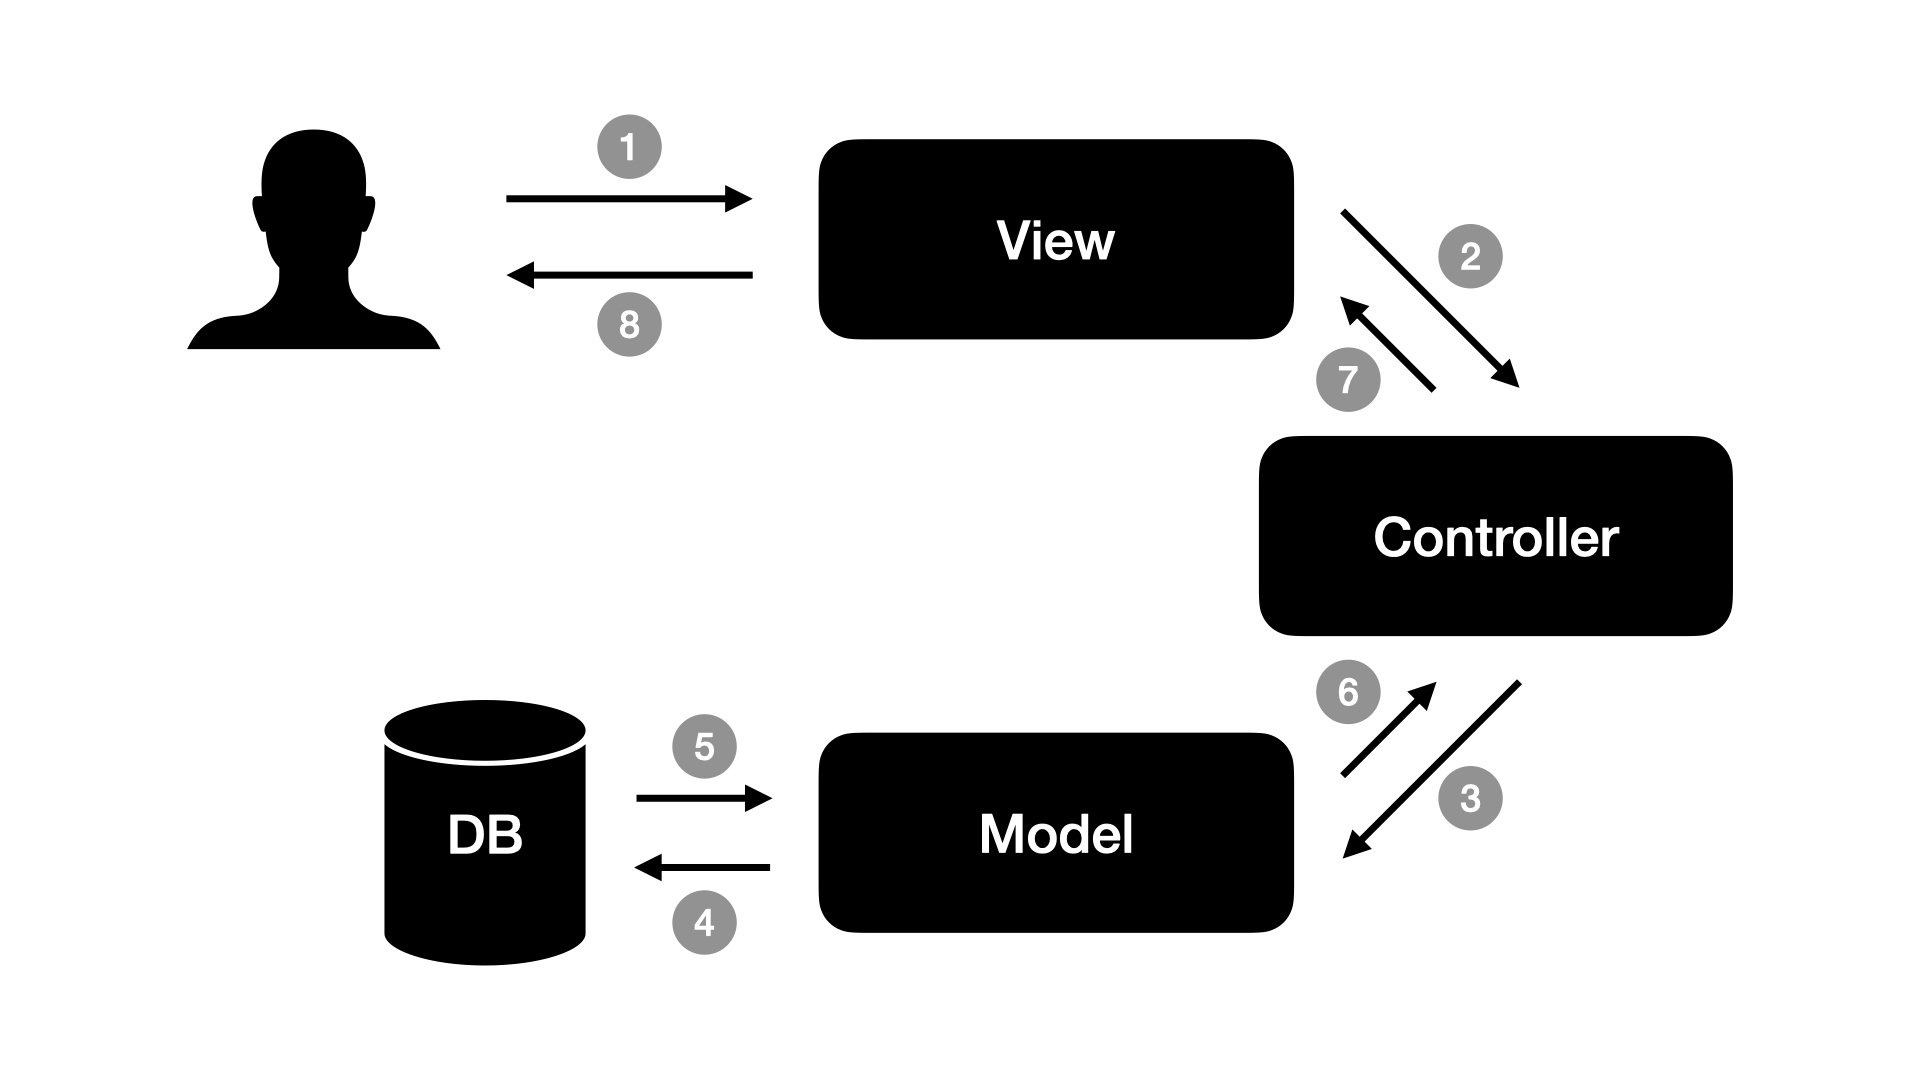
\includegraphics[width=.6\textwidth]{Assets/Interaktionsorientiert.001}
	\caption[Kommunikation zwischen Controller und Model]{Kommunikation zwischen Controller und Model, \\ (1) Der Benutzer sieht die graphische Darstellung und führt eine Aktion aus (2). Der Controller verarbeitet die Aktion und ruft über das Model Daten ab (3). Das Model greift auf die Datenbank zu und lädt die entsprechenden Informationen (4 und 5). Anschließend gibt das Model die Inhalte an den Controller zurück (6). Dieser gibt die Daten an die View weiter (7), welche abschließend die neuen Inhalte dem Benutzer anzeigt (8).}
	\label{fig:mvc-cm-kommunikation}
 \end{figure}
 
 \begin{figure}
 	\centering
    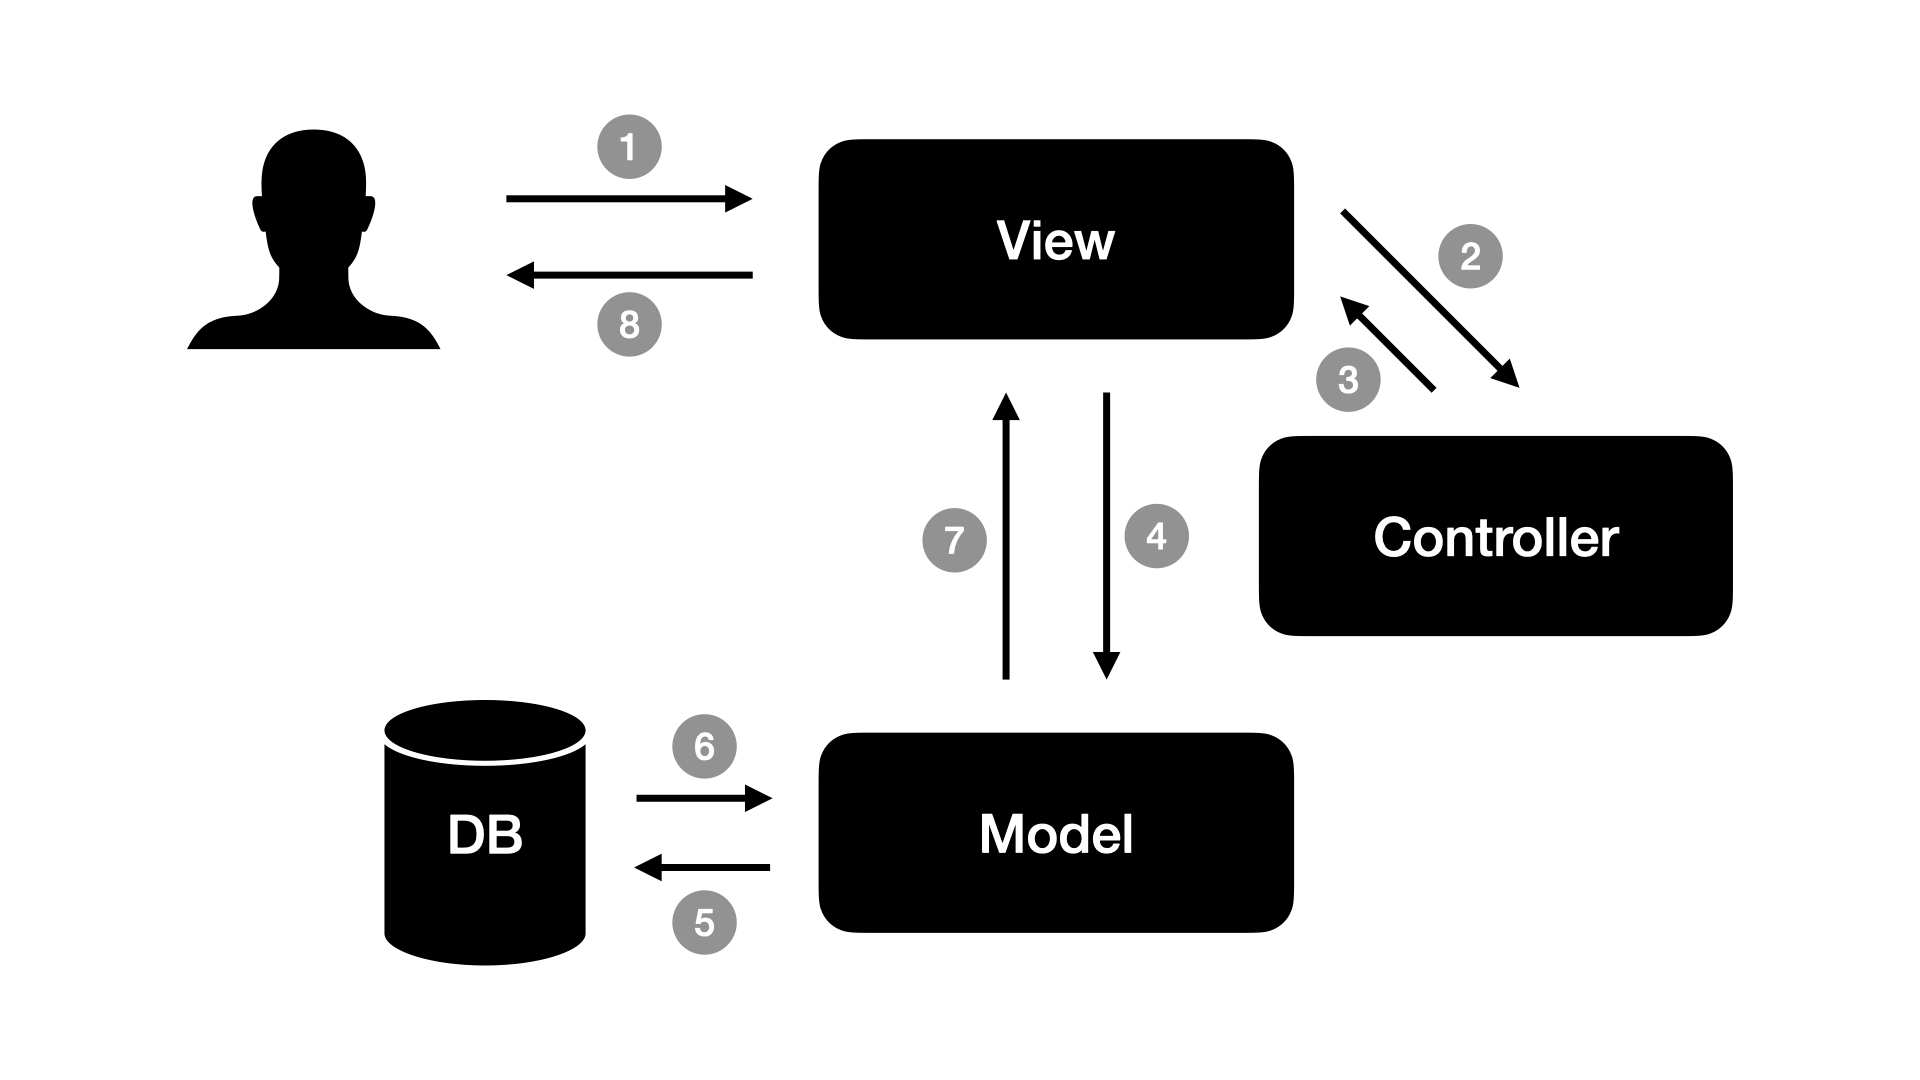
\includegraphics[width=.6\textwidth]{Assets/Interaktionsorientiert.002}
	\caption[Kommunikation zwischen View und Model]{Kommunikation zwischen View und Model, \\ (1) Der Benutzer sieht die graphische Darstellung und führt eine Aktion aus (2). Der Controller verarbeitet die Aktion und rendert umgehend die graphische Darstellung (3). Die View lädt über das Model die Daten (4). Das Model greift auf die Datenbank zu und lädt die angeforderten Informationen (5 und 6). Anschließend gibt es die Inhalte an die View zurück (7). Dieses zeigt abschließend die neuen Inhalte dem Benutzer anzeigt (8).}
    \label{fig:mvc-vm-kommunikation}
 \end{figure}

\subsubsection{REST-Architektur}
\label{sec:rest}

Neben den bislang genannten Architekturstilen, gibt es eine Vielzahl von weiteren Strukturierungen, die sich erst in den letzten 20 Jahre entwickelt haben. Einer dieser Architekturstile ist die REST-Architektur, welche vom Miterfinder des HTTP-Standards Roy Fielding definiert wurde \parencite[][S. 128]{starke_effektive_2015}. Er beschrieb diesen Stil in seiner Dissertation an der Universität von Kalifornien im Jahr 2000 und charakterisiert ihn als Architekturstil für das Web.

Dabei steht REST für \textit{Representational State Transfer}, welches einen Architekturstil für verteilte Systeme beschreibt und auf der Client-Server-Architektur aufbaut \parencite[][S. 76]{fielding_architectural_2000}. Client-Server-Architektur beschreibt eine Ausprägung eines verteilten Systems, bei dem die Anwendung in Server und Clients geteilt werden \parencite[][S. 117]{starke_effektive_2015}.\footnote{Dabei beziehen sich die Begriffe \textit{\enquote{Server}} und \textit{\enquote{Client}} auf Software Komponenten und auf den physischen Server und das Endgerät des Nutzers (Client). Des Weiteren grenzt sich der Architekturstil von der Mainframe Architektur ab, bei der über Terminals Anweisungen an einen Großrechner gestellt werden.}

Ein Server ist dabei eine Software Komponente im Netzwerk, welche Services anbietet. Ein Service könnte beispielsweise zuständig sein, alle Informationen der hinterlegten Kunden auszugeben. Der Client hingegen konsumiert lediglich diese Informationen und dient dem Benutzer als Bedienungsoberfläche. Dies bedeutet, dass der Server nur passiv auf Anfragen vom Client wartet, während der Client selbst keine Informationen verarbeitet, sondern ausschließlich anzeigt. Gleichwohl handelt es sich um ein Programm, welches auf dem Endgerät des Benutzers (Computer, Mobiltelefon) ausgeführt wird.

Die REST-Architektur verwendet diese Aufteilung, um eine feste Trennung der Zuständigkeit zu integrieren \parencite[vgl.][S. 78]{fielding_architectural_2000}.

Die zweite Bedingung, die Fielding an den Architekturstil stellt, ist dass die Kommunikation zustandslos, zu Englisch (stateless), abläuft \parencite[][S. 78]{fielding_architectural_2000}. Dies bedeutet, dass die Nachrichten, die zwischen Server und Client ausgetauscht werden, alle nötigen Informationen beinhalten \parencite[][S. 128]{starke_effektive_2015}. Somit gibt der Server auf Anfrage des Clients stets die gleiche Antwort zurück, egal ob dieser zum Ersten, oder zum wiederholten Mal angefragt wurde. Des Weiteren hängt die Antwort nicht vom Client ab.
Diese Entkopplung zwischen den Komponenten ermöglicht, dass die Aufgabe des Servers, sowie des Clients durch mehrere Computer verrichtet werden kann und  das System skalierbar ist \parencite[][S. 79]{fielding_architectural_2000}.

Der Hauptunterschied zwischen der REST-Architektur und anderen Stilen, liegt in der genauen Bestimmung der zu verwendenden Kommunikationsschnittstellen. So bestimmt die REST-Architektur sehr explizit, welche Form zur Kommunikation verwendet werden darf. So werden Methoden vom Server über HTTP-Standards aufgerufen. Konkret bedeutet dies, dass die einzelnen Dienste des Servers sich nach den HTTP-Methoden (GET, PUT, POST und DELETE) richten und es ein klares Mapping zwischen ihnen gibt. \parencite[vgl.][S. 128]{starke_effektive_2015}. Somit baut die REST-Architektur auf einem Kommunikationsstandard auf, der sich im Internet etabliert hat.

Auf Grundlage der standardisierten Kommunikation können zwischen Server und Client intelligente Zwischenstationen geschaltet werden, die dafür zuständig sind, häufig vorkommende Anfragen abzuspeichern \parencites[vgl.][S. 79 f.]{fielding_architectural_2000}[][S. 128]{starke_effektive_2015}.

Die Antwort des Servers erfolgt durch Repräsentationen der Daten, wovon es für jede Ressource\footnotemark mehrere Formate gibt. So kann eine Schnittstelle abhängig vom Aufruf sowohl JSON, als auch XML oder HTML zurückgeben \parencite[vgl.][S. 128]{starke_effektive_2015}.
\footnotetext{Als Ressource werden die Informationen bezeichnet, die durch den Aufruf einer URL zurück gegeben werden. Ein Beispiel wäre der HTTP-Aufruf \textit{GET: https://api.plurapolit.de/api/users}, der alle Informationen der User zurück sendet.}

Verwendet wird die REST-Architektur ausschließlich für Anwendungen im Internet, da es auf die Anwendung des Hypertext Transfer Protokoll\footnote{Weitere Informationen zum Hypertext Transfer Protokoll kann unter folgender Literatur gefunden werden \parencite{leach_hypertext_2020}.} (HTTP) angewiesen ist. Dabei findet der Architekturstil sowohl Anwendung für ganze Systeme, als auch in komplexen Anwendungen mit einer Vielzahl einzelner Services.

\subsubsection{Monolithische Architektur}
\label{sec:monolith}

Der Begriff \textit{\enquote{Monolith}} leitet sich vom altgriechischen \textit{\enquote{monólithos}} ab und bedeutet \textit{\enquote{aus einem Stein}} \parencites[vgl.][]{duden_nodate}[vgl.][]{dwds_nodate}. In der Gesteinskunde wird damit ein natürlich entstandener Gesteinsblock bezeichnet, der komplett aus einer Gesteinsart besteht \parencite[vgl.][]{dwds_nodate}.

Nach Rod Stephens liegt eine monolithische Softwarearchitektur vor, wenn jegliche Funktionalität des Systems miteinander verbunden ist. Dabei spricht er über die Verbindung von Dateneingabe, Datenausgabe, Datenverarbeitung, sowie Fehlerhandhabung und Benutzeroberflächen \parencite[vgl.][S. 94]{stephens_beginning_2015}.

Anders sieht es Sam Newman. Nach ihm liegt ein monolithisches System schon dann vor, wenn die gesamte Funktionalität eines Systems gemeinsam über einen Deployment-Prozess\footnotemark bereitgestellt wird \parencite[vgl.][Kap. 2.2]{newman_monolith_2019}. Folglich muss nicht zwingend jegliche Logik miteinander verbunden sein. Er unterteilt monolithische Systeme in drei Kategorien: Einzelprozess Monolithe, modulare Monolithe und verteilte Monolithe \parencite[vgl.][Kap. 2.2]{newman_monolith_2019}.
\footnotetext{Deployment-Prozess, oder auch Bereitstellungsprozess, bezeichnet den Prozess ein Software-System Benutzern zur verfügung zustellen \parencite[vgl.][]{softwareverteilung_2020}.}

Der Einzelprozess Monolith ist die gängigste Form und deckt sich mit der Definition von Rod Stephens. Es handelt sich dabei, um ein System bei dem das gesamte System einen Prozess abbildet. Dies bedeutet, dass jegliche Funktionalität aufeinander aufbauend ist und nur eine Datenspeicherung für die gesamte Anwendung verwendet wird \parencite[vgl.][Kap. 2.2.1]{newman_monolith_2019}.

Anders ist dies beim modularen Monolith. Er zeichnet sich darin aus, dass die Funktionalität in einzelne Module geteilt wird, die eine separate Datenspeicherung besitzen können \parencite[vgl.][Kap. 2.2.2]{newman_monolith_2019}. Im Gegensatz zu verteilten Systemen sind die einzelnen Module jedoch nicht auf separaten Computern verteilt, sondern über einen Rechner online gestellt. Des Weiteren sind die einzelnen Module nur leicht entkoppelt, sodass es zwischen ihnen Abhängigkeiten geben kann.

Dies ist bei verteilten Monolith anders, da die einzelnen Module komplett entkoppelt sind und Nachrichten ausschließlich über definierte Schnittstellen ausgetauscht werden \parencite[vgl.][S. 116]{starke_effektive_2015}. Ein verteilter Monolith erfüllt somit jegliche Anforderungen an ein verteiltes System mit der Ausnahme, dass alle Komponenten durch nur einen Prozess online gestellt werden.

Weder Stephens noch Newman geben Vorgaben hinsichtlich der Gliederung innerhalb eines monolithischen Systems. Demnach kann ein Model-View-Controller-Ansatz als monolithisches System gelten, solange es einheitlich bereitgestellt wird.

Im Rahmen dieser Arbeit wird beim Begriff Monolith stets von einem Einzelprozess Monolith ausgegangen, außer es wird expliziert von einem modularen, oder verteilten Monolithen geschrieben.

Vergleicht man das monolithische System mit einem verteilten System, gibt es Vor- und Nachteile \parencite[vgl.][Kap. 2.2.4 und Kap. 2.2.5]{newman_monolith_2019}. So ist das Bereitstellen eines Monoliths einfacher, da es einen Bereitstellungsprozess für die gesamte Anwendung gibt. Wiederum führt dies dazu, dass der Prozess deutlich länger dauert. Diese Tatsache ist besonders dann gravierend, wenn vermehrt kleine Änderungen vorgenommen werden. Andererseits vereinfacht eine Anwendung, die als ein Prozess zu sehen ist, die Fehlersuche und ermöglicht es Funktionen mehrfach zu verwenden. Das verursacht jedoch, dass schnell Abhängigkeiten entstehen können und Änderungen ungewollte Fehler verursachen. Dadurch wird die Umsetzung von neuen Funktionen mit steigender Codemenge verlangsamt und der Einstieg von neuen Teammitgliedern erschwert.

Da alle Entwickler eines Unternehmens auf einer Codebase arbeiten, kommt es schnell zu Unterschieden im Programmcode. So führt ein Monolith dazu, dass bei einer großen Anzahl von Entwicklern viele Absprachen notwendig sind \parencite[vgl.][Kap. 2.2.4]{newman_monolith_2019}.

Anders ist es bei systemübergreifenden Tests: Diese werden durch ein monolithisches System begünstigt und können im Vergleich zu einem verteilten System einfacher umgesetzt werden  \parencite[vgl.][Kap. 2.2.5]{newman_monolith_2019}.

\subsubsection{Einordnung des aktuellen Systems von PluraPolit}
\label{sec:einordnung}

Wie bereits in der Einleitung beschrieben, bietet PluraPolit eine Plattform an, die Jung- und Erstwählern bei der politischen Bildung unterstützt.

Es wurde ein Software-System entwickelt, welches auf der einen Seite PluraPolit die Möglichkeit gibt, Content zu verwaltet und auf der anderen Seite den Endkunden die Inhalte graphisch aufbereitet. Hierfür wurde, neben der Plattform für die Nutzer, ein Content Management System (CMS) umgesetzt. Programmiert wurde dieses in der Programmiersprache Ruby on Rails.\footnote{
Ruby on Rails, kurz auch als Rails bezeichnet, ist ein quellenoffenes Webframework, welches für die Programmiersprache Ruby entwickelt wurde \parencites[vgl.][S.4]{hartl_ruby_2016}{ruby_org}[vgl.][S. 24]{sieben_wochen}. Es ist komplett Open Source und wird von einer aktiven Community entwickelt. Es gibt eine Vielzahl von kostenfreien Paketen, sogenannte Gems, die nach Belieben zu einem Projekt hinzugefügt werden können. Im Vergleich zu anderen Frameworks zeichnet sich Rails besonders durch seine Implementierung der REST-Architektur aus \parencite[vgl.][S. 5]{hartl_ruby_2016}. Diese Implementierung führt jedoch dazu, dass eine Vielzahl von Bedingungen an die Entwicklung und Implementierung von Rails Anwendungen gestellt werden. Getreu dem Motto \textit{\enquote{Konvention vor Konfiguration}} nutzt Rails die Bestimmungen als Vorteil und integriert ein System, in das externe Pakete ohne Konfigurationsaufwand hinzugefügt werden können \parencite{ruby_doctrine}.
} Strukturiert werden Rails Anwendungen nach dem Model-View-Controller-Ansatz \parencites[vgl.][S. 66 ff.]{hartl_ruby_2016}.

\begin{figure}
	\centering
	\begin{subfigure}[a]{0.4\linewidth}
		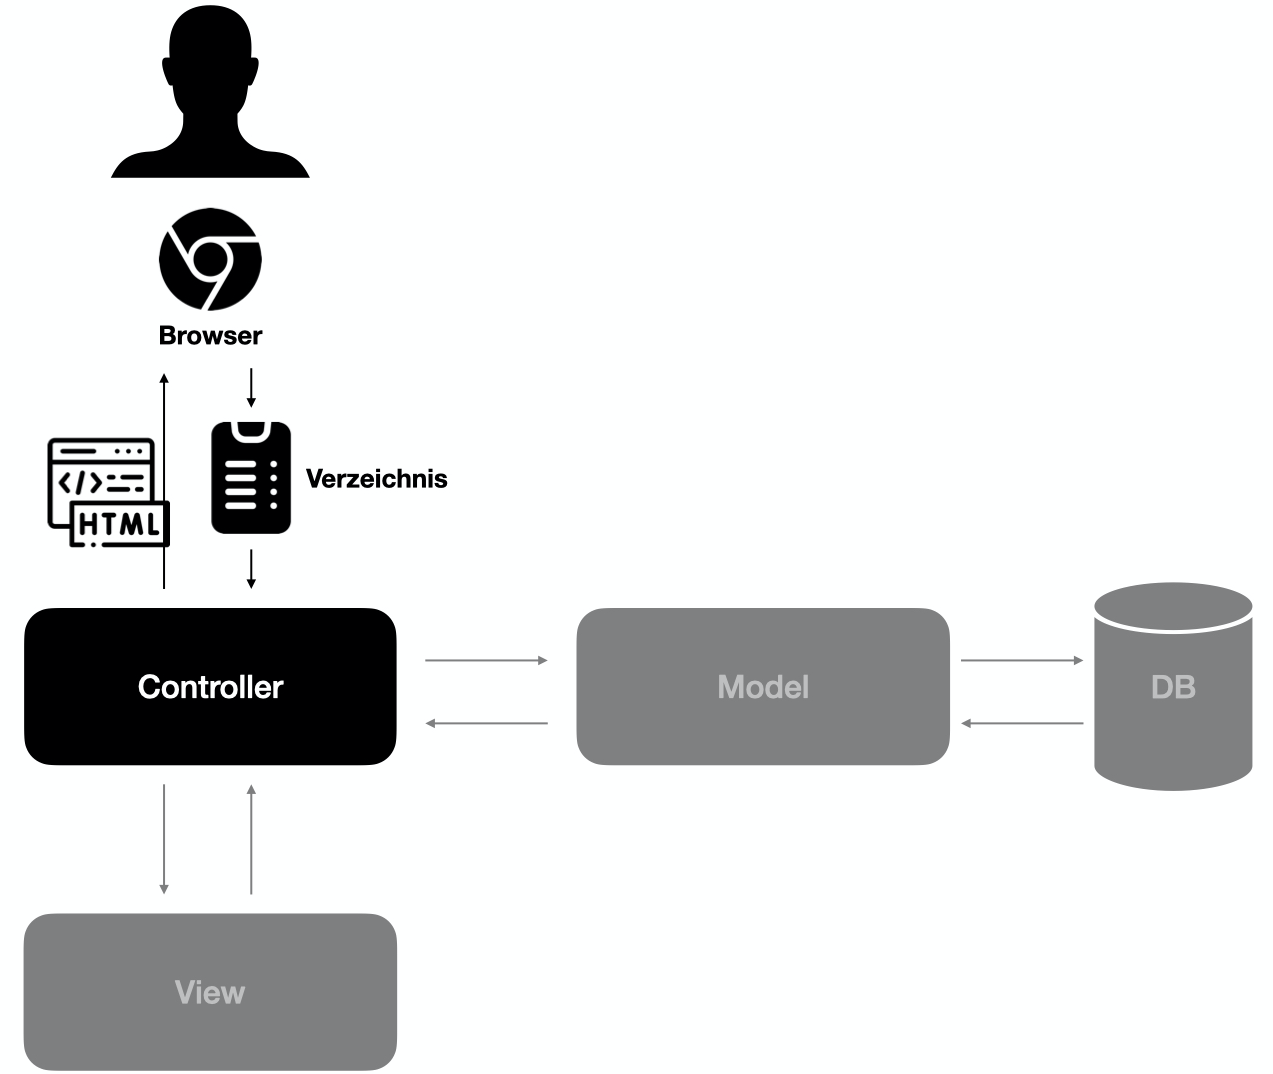
\includegraphics[width=\linewidth]{Assets/PluraPolit-Softwaresystem.001}
		\caption{Aufruf der Webseite}
		\label{fig:plurapolit-call-webpage}
	\end{subfigure}
	\begin{subfigure}[a]{0.4\linewidth}
		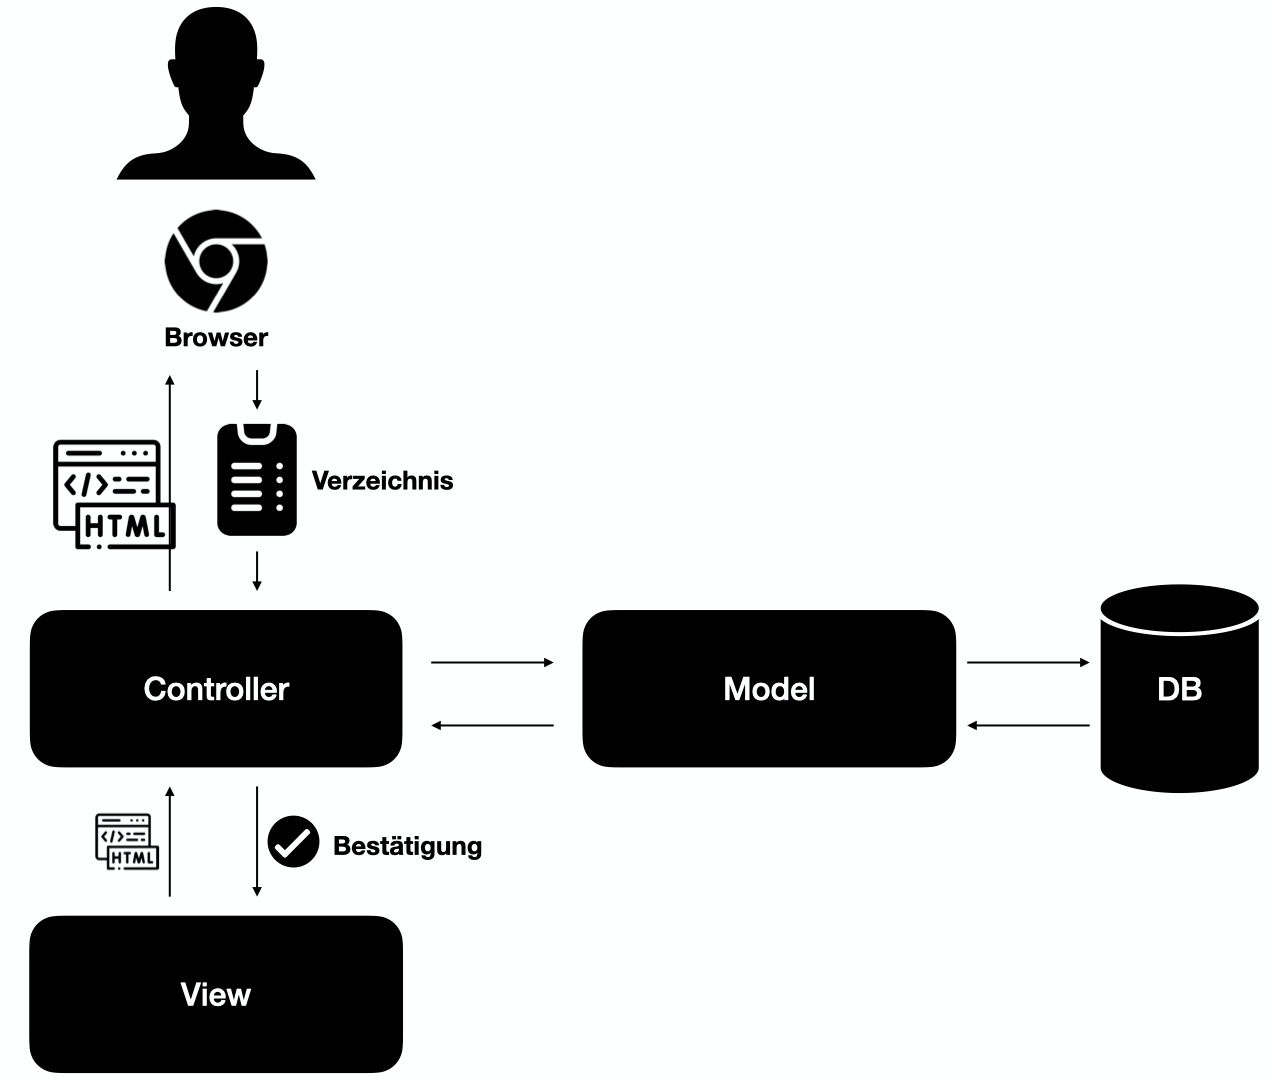
\includegraphics[width=\linewidth]{Assets/PluraPolit-Softwaresystem.002}
		\caption{Abspeichern der Tondatei}	
		\label{fig:plurapolit-save-sounddatei}
	\end{subfigure}
	\begin{subfigure}[b]{0.4\linewidth}
		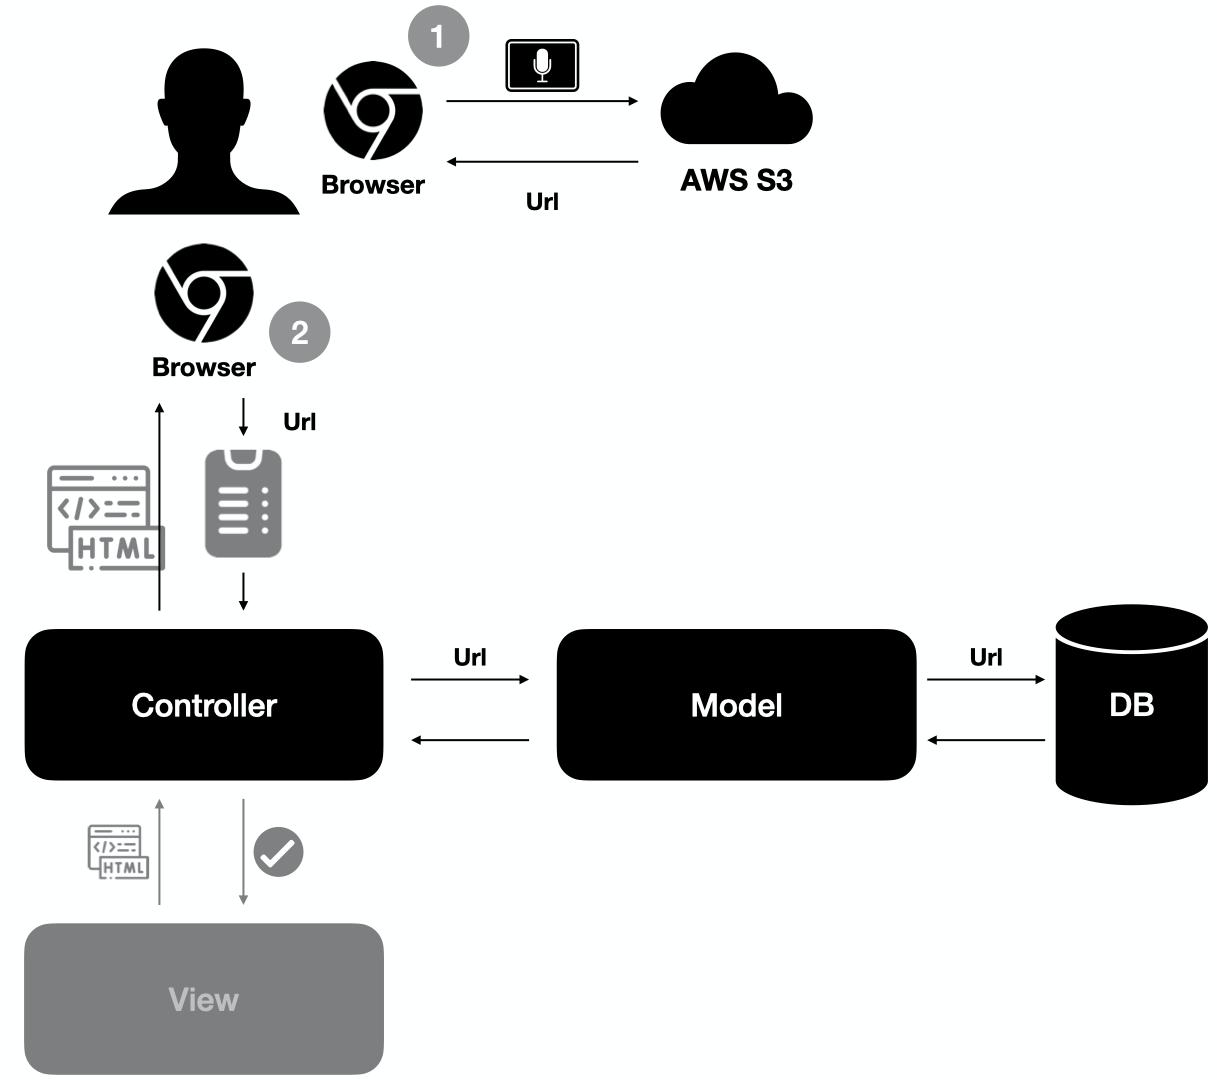
\includegraphics[width=\linewidth]{Assets/PluraPolit-Softwaresystem.003}
		\caption{Speichern zu S3}
		\label{fig:plurapolit-save-to-s3}
	\end{subfigure}
	\caption{Speichern einer Tonaufnahme}
	\label{fig:coffee}
\end{figure}

Um eine neue Tonaufnahme einzupflegen wird, die entsprechende Webseite im Browser aufgerufen. Dabei sendet der Browser über die URL eine Anfrage an den Server, der anhand eines Verzeichnis den verantwortlichen Controller bestimmt und die Anfrage an diesen weiterleitet.  Der Controller verarbeitet die Anfrage und schickt eine HTML-Seite zurück (siehe \cref{fig:plurapolit-call-webpage}).

Über diese Webseite kann die Aufnahme hochgeladen und abgespeichert werden. 
Dies geschieht, indem per Klick im CMS ein HTTP-Anfrage an den Controller geschickt wird. Der Controller speichert den Eintrag und bestätigt das erfolgreiche Abspeichern im View. Das Speichern geschieht dabei über das Model (siehe \cref{fig:plurapolit-save-sounddatei}).

Dabei wird die Tondatei selbst nicht in der Datenbank gespeichert, sondern lediglich ein Verweis darauf. 
Die Datei wird vorher zum Speicherservice von Amazon Web Services (S3) geladen, welcher die Tonaufnahme über eine URL zur Verfügung stellt. Nur die URL wird in die Datenbank hinterlegt (siehe \cref{fig:plurapolit-save-to-s3}).

\begin{figure}
	\centering
	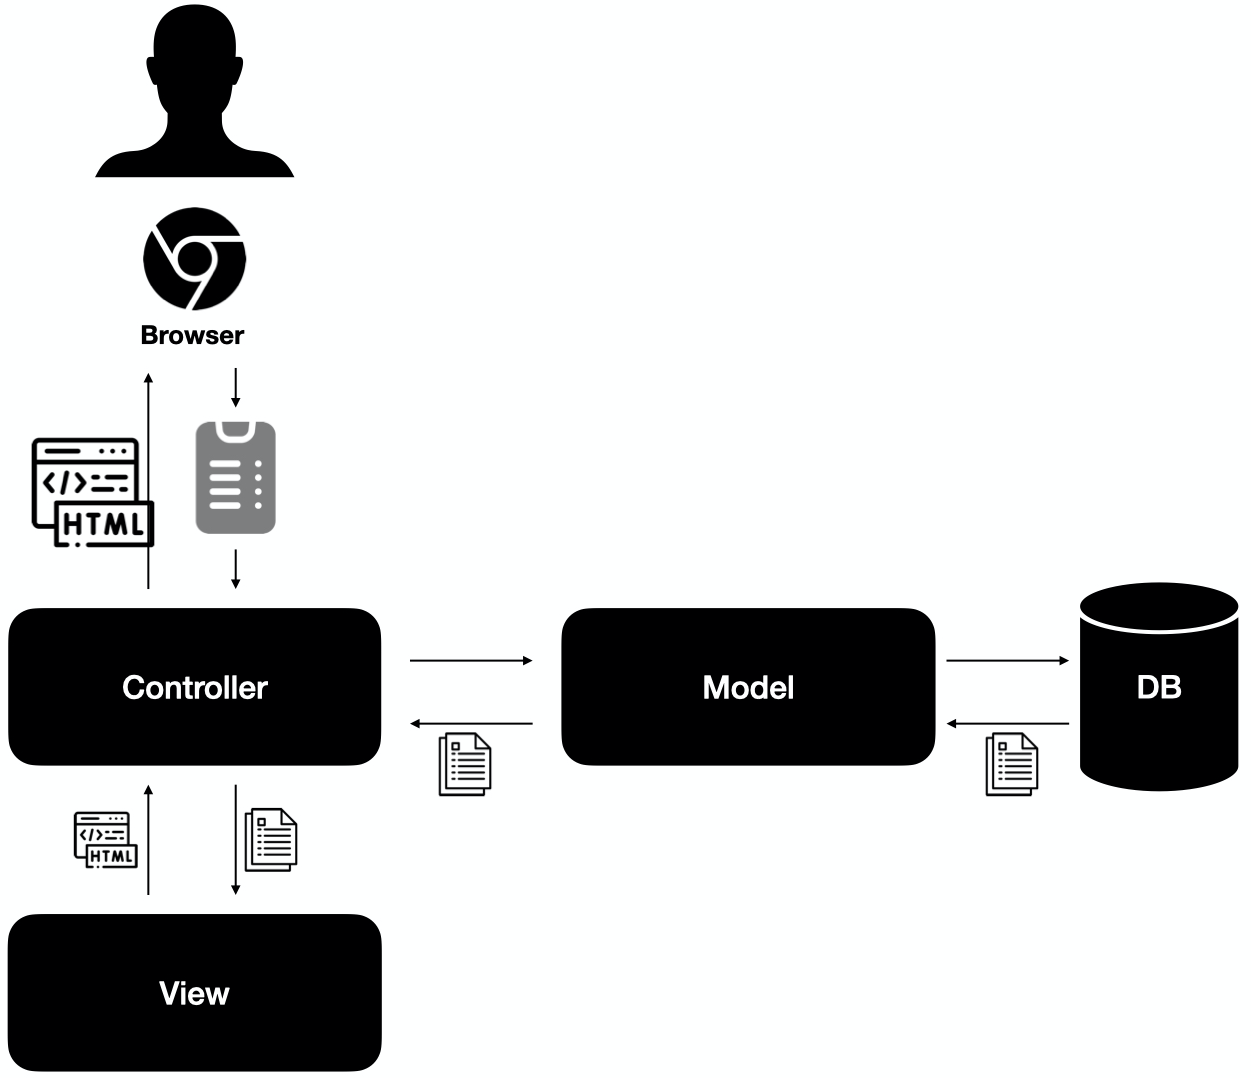
\includegraphics[width=0.5\linewidth]{Assets/PluraPolit-Softwaresystem.004}
	\caption{Inhalte bearbeiten}
	\label{fig:plurapolit-edit}
\end{figure}

Neben dem Abspeichern der Tonaufnahmen kann das CMS auch zum Bearbeiten und Anpassen von bestehenden Datensätzen genutzt werden. Hierfür wird die jeweilige Webseite aufgerufen, welches dazu führt, dass der Controller die angeforderten Daten aus der Datenbank lädt und die entsprechende graphische Darstellung an den Browser zurück gibt. Dabei greift der Controller nicht direkt auf die Datenbank zu, sondern lädt die Inhalte über den Model.
Auch übergibt der Controller lediglich die geladenen Inhalte an die View, welche  die Daten über Embedded RuBy in HTML integriert und die fertige Webseite  an den Controller zurück gibt (siehe \cref{fig:plurapolit-edit}).

\begin{figure}
	\centering
	\begin{subfigure}[c]{0.3\linewidth}
		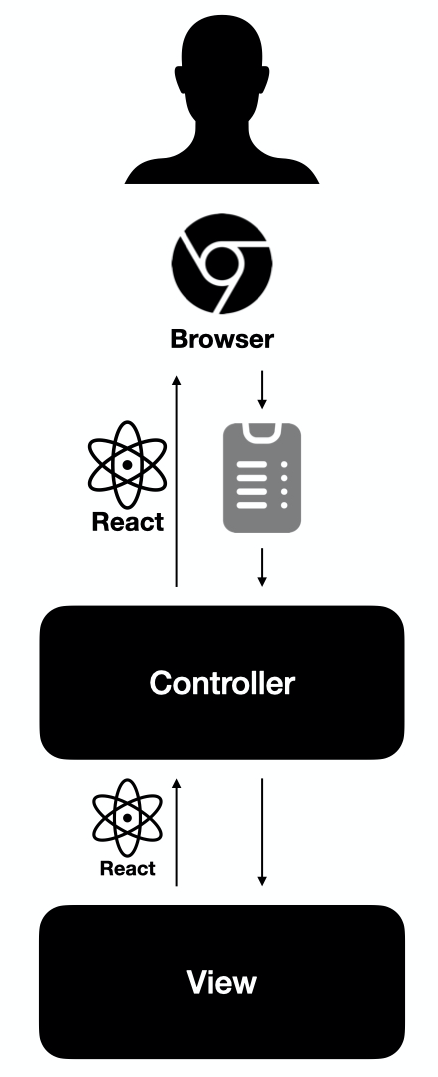
\includegraphics[,height=7cm]{Assets/PluraPolit-Softwaresystem.005}
		\caption{React-App aufrufen}
		\label{fig:plurapolit-load-react}
	\end{subfigure}
	\begin{subfigure}[c]{0.6\linewidth}
		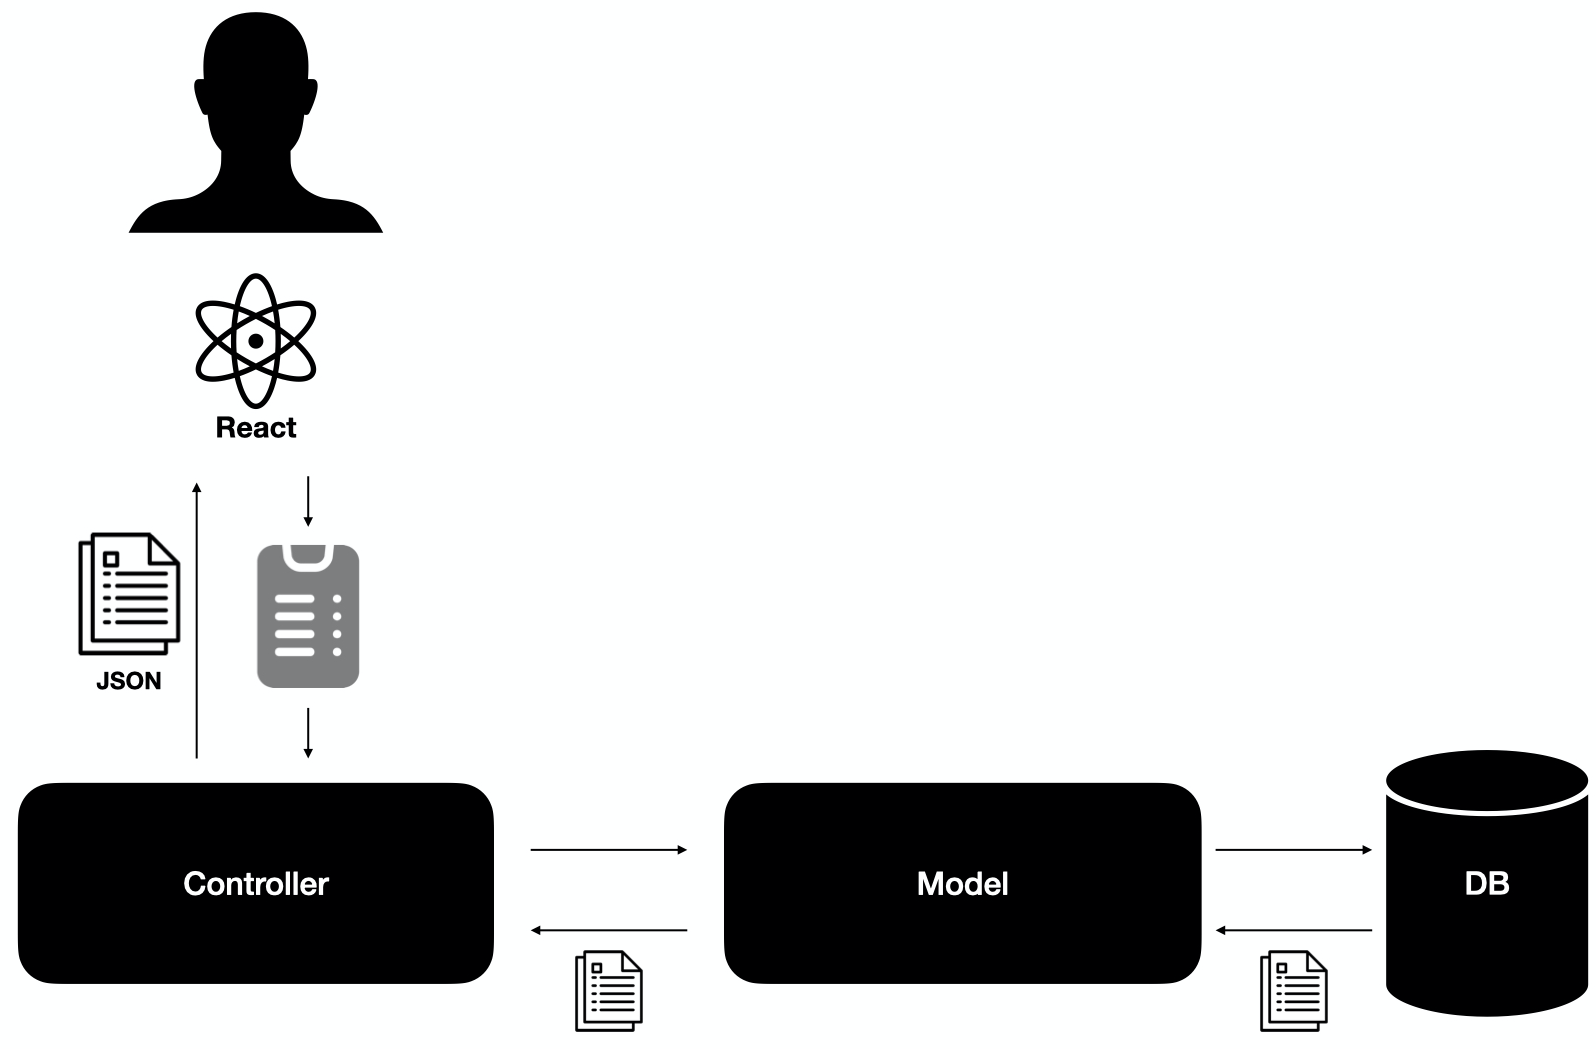
\includegraphics[width=\linewidth]{Assets/PluraPolit-Softwaresystem.006}
		\caption{React-App lädt Inhalte}
		\label{fig:plurapolit-react-data}
	\end{subfigure}
	\caption{Endkunde lädt die Plattform}
\end{figure}

Bei der Plattform für die Endkunden handelt es sich, um die selbe Anwendung wie beim CMS, mit dem Unterschied, dass die graphischen Darstellung durch eine React-Anwendung übernommen wird. So wird beim Aufruf der Plattform eine Anfrage an den Controller geschickt, der anschließend die kompilierte React-Anwendung zurück gibt (siehe \cref{fig:plurapolit-load-react}).

Diese lädt eigenständig jegliche Informationen über HTTP-Anfragen und kümmert sich um interne Seitenaufrufe. Die Anfragen werden dabei asynchron an die Rails Applikation geschickt und vom Controller beantwortet. Somit erhält die React-Anwendung über die Kommunikation von Controller und Modul, den Content aus der Datenbank, der vorher eingepflegt wurde (siehe \cref{fig:plurapolit-react-data}).

Es gibt also eine Aufteilung bezüglich der graphischen Darstellung in Content Management System und Plattform. Die Datenspeicherung und Verwaltung sind jedoch gleich. Die gesamte Codebase wird in einem Bereitstellungsprozesses dem Hosting Service zur Verfügung gestellt. Damit handelt es sich bei dem System von PluraPolit um ein Monolith, welches teilweise modular ist, die REST-Standards erfüllt und nach dem Model-View-Controller-Ansatz strukturiert ist. Des Weiteren nutz das System vereinzelt externe Services von AWS, um Tondateien zu speichern.


\subsection{Microservices}

Nachdem nun die einzelne Architekturstile vorgestellt wurden und das System von PluraPolit eingeordnet wurde, wird nun Microservices vorgestellt.

Dabei handelt es sich um eine Architekturstil, der ein Vertreter der verteilten Systeme ist und sich historisch aus der Service Orientierten Architektur abgeleitet hat (siehe \cref{sec:Zielsetzung}).

Eberhard Wolff beschreibt Microserivces als Ansatz Software in einzelne Module zu teilen und definiert es als Modularisierungskonzept, welches Einfluss auf die Unternehmesorganisation und Software-Entwicklungsprozess hat \parencite[vgl.][Kap. 1.1]{wolff_microservices_2018}. Dabei ist jedes Module ein eigenes Programm.

Sam Newman schließt sich Wolff an und beschreibt Microservices als voneinander unabhängig einsetzbare Dienste, die um eine Geschäftsdomäne herum modelliert sind \parencite[vgl.][Kap. 2.1]{newman_monolith_2019}.

Somit beschreiben beide Microservices als ein System aus einzelnen unabhängigen Services, die sich an ein Geschäftsdomäne richten. Insbesondere die Abhängigkeit zum Geschäftsprozess wird nachfolgend näher beschrieben.

\subsubsection{Zusammenhang und Verknüpfung}

Wenn es um das aufteilen von Software geht, ist es wichtig zu verstehen wie die einzelnen Funktionen und Klassen zusammenhängen und welche Verknüpfungen es zwischen ihnen gibt.

Dabei bezieht sich der Zusammenhang auf die funktionale Abhängigkeit zweier Funktionen oder Klassen \parencite[vgl.][Kap. 2.3.1]{newman_monolith_2019}. Somit liegt ein hoher Zusammenhang vor, wenn Quellcode anhand seiner logischen Zugehörigkeit geordnet ist. Eine konkrete Umsetzung dieses Bestreben ist im Abschnitt zum Model-View-Controller-Ansatz zu finden.

Verknüpfung hingegen beschreibt in welchem Maß, Funktionen und Klassen verbunden sind, ohne dass sie logisch zusammen gehören \parencite[vgl.][Kap. 2.3.2]{newman_monolith_2019}. Somit bezieht sich Verbindung ausschließlich auf eine technisch vorliegende Kopplung. Ein typisches Beispiel hier für ist, wenn ein Datenabruf an mehreren Stellen direkt über das Datenbankschema abläuft. Dadurch entsteht eine Abhängigkeit auf das Schema, sodass falls sich das Schema ändert auch die jeweiligen Aufrufe geändert werden müssen.

Insbesondere in monolithischen Systemen können viele Verknüpfungen entstehen, da keine festen Abgrenzungen zwischen einzelnen logischen Bereiche definiert sind. Somit kann es sein, dass ein Monolith, welches historisch wächst, keine klare Struktur aufzeigt. Es entsteht hieraus ein System, welches anfällig für Veränderungen ist.

Für ein Microservicesarchtektur ist jedoch das Bestreben klare Abgrenzung zu erlangen, und einzelne stabile Services zu etablieren. Diese sollen soweit es geht von einander entkoppelt funktionieren. Somit ist das Ziel für eine Microservicearchitektur einen hohen Zusammenhang bei geringer Verknüpfung zu besitzen. Dabei ist dies nicht nur die Zielsetzung für Microservices allgemein, sondern ein generelles Bestreben für stabile Systeme.\footnote{Dies bezieht sich auf das Gesetz von Constantine, welches besagt \textit{\enquote{A structure is stable if cohesion is strong and coupling is low.}} \parencite[S. 43]{endres_handbook_2003}.} Für Microservices bedeutet dies Konkret, dass ein Services ausschließlich aus funktional abhängigem Quellcode besteht und technische Implementierungen, wie zum Beispiel Datenbankstrukturen und Funktionsaufrufe, hinter klar definierten Schnittstellen versteckt sind.

\subsubsection{Conway's Law}

Die Abhängigkeit der Kommunikationsstruktur im Unternehmen zur verwendeten Software Architektur.

\begin{itemize}
	\item Begriff erklären
	\item Auswirkungen für die Teamstruktur beschreiben
\end{itemize}

\subsubsection{Bounded Contexts}

An diesem Punkt sollte eine Definition des Begriffes Bounded Contexts gegeben werden. Dies ist insbesondere wichtig, da Domain Driven Design darauf aufbaut und Bounded Contexts umsetzt.

\subsubsection{Domain Driven Design}

\begin{itemize}
	\item Was ist DDD?
	\item Was sind Bounded Contexts?
	\item 	Bespiele dazu.
	\item Schlussfolgerung für PluraPolit
\end{itemize}


\subsection{Microservice}

Wie aus dem vorhergehenden Abschnitt hervor geht sind Microservices einzelne, unabhängige Services, die um eine Geschäftsdomäne modelliert sind, welche auf Grundlage der klaren Schnittstellen entkoppelt und durch einzelne Kontext begrenzt sind. Die Kontexte ermöglichen das Verwenden von Service internen Terminologie und Verwendung ausschließlich benötigter Daten. Abschließend hat \cref{sec:conway} gezeigt, dass nur ein Team für ein Service zuständig ist.

In seinem Buch \textit{Monolith to Microservices} geht Newman darauf ein, dass wohl die wichtigste Eigenschaft von einem Microservice die unabhängige Einsetzbarkeit ist \parencite[vgl.][Kap. 2.1.1]{newman_monolith_2019}. Er sieht darin die Verkörperung von Unabhängigkeit und eigenständigen Teams, welche durch die Kommunikation der Services durch standardisierte Schnittstellen ermöglicht wird. Die meist verbreitete Art der Schnittstelle ist die nach dem REST-Standard, welche sich an eine Kommunikation über HTTP richtet (siehe \cref{sec:rest}).
 
Da viele Programmiersprachen den Informationsaustausch über HTTP ermöglichen, ist ein Microservice unabhängig einer bestimmten Technologie. Somit kann jedes Team eigenständig entscheiden, welche Programmiersprache sie verwenden wollen \parencite[vgl.][Kap. 1.2]{wolff_microservices_2018}. Dadurch können Sprachen nach Präferenz und Problemstellen gewählt werden, ohne dass eine Inkompatibilität zum Rest des Systems entsteht.

Vielmehr ermöglicht der Austausch über standardisierten Kommunikationswege, dass Services erstellt werden, die austauschbar sind \parencite[vgl.][Kap. 1.2]{wolff_microservices_2018}. Somit können zum Beispiel einige Services durch Dienste von Drittanbieter ausgeführt werden und Entwicklungskosten gespart werden. Außerdem wird dadurch die Möglichkeit geschaffen auf bestehender Logik aufzubauen und ältere Systeme mit modernen Technologien zu verbinden.

\cref{sec:ddd} hat gezeigt das Kontextgrenzen Microservices es ermöglicht Daten nach eigenem ermessen zu benennen und zu verwalten. Konkret besitzt jeder Dienst eine eigene Datenspeicherung, in Form zum Beispiel eines File-Storage-Systems oder einer Datenbank \parencite[vgl.][Kap. 2.1.3]{newman_monolith_2019}. Für das Gesamtsystem bedeutet dies, dass keine einheitliche Datenspeicherung vorliegt, sondern jeder Service die notwendigen Informationen verwaltet. Um jedoch die Funktionalität des gesamten Systems zu erhalten, müssen im Vorfeld bestimmt werden, wie der Informationsaustausch zwischen den Services abläuft \parencite[vgl.][Kap. 4.1]{wolff_microservices_2018}. Hierfür ist es wichtig zu bestimmen, welche Services welche Informationen verwalten und falls Abhängigkeiten zu anderen Diensten bestehen, die Schnittstellen festzulegen. Insbesondere die genauen Endpunkt und die zu erwarteten Informationen müssen bestimmt werden. Die Handhabung innerhalb eines Services, ist dann wieder dem einzelnem Team überlassen. 

Gibt es ein Service, der Informationen von einem anderen Dienst benötigt, fordert dieser die Daten über öffentliche Schnittstellen aktive an. Dies führt jedoch dazu, dass gleiche Informationen von mehrere Diensten verwaltet werden und es zu unterschieden Datenständen kommt \parencite[vgl.][Kap. 4.1]{wolff_microservices_2018}. Es entsteht die Herausforderung Informationen zwischen Services Konsistent zu halten (siehe \cref{sec:cap}).

Volle Unabhängigkeit eines Microservice kann nur erreicht werden, wenn dieser auch für die Benutzeroberfläche verantwortlich ist \parencite[vgl.][Kap. 4.4]{wolff_microservices_2018}. In der Praxis ist dies jedoch schwierig, da eine Webseite Inhalte von mehreren Services anzeigt. Insbesondere nachdem AngularJS\footnote{AngularJS ist ein JavaScript Framework, welches 2010 von Google entwickelt wurde und eine Open-Source-Software ist \parencite{angularjs}.} veröffentlicht wurde, gibt es immer mehr JavaScript Frameworks die um die Benutzererfahrung zu verbessern mehr Logik in das Frontend legen. React.js ist eines dieser Frameworks. Die Beliebtheit hinter diesen Frameworks, liegt darin, dass jede einzelne Webseite nicht mehr als einzelne Seite betrachtet wird, sondern Informationen zwischen Benutzeroberflächen hinweg verwaltet werden \parencite[vgl.][Kap. 9.1]{wolff_microservices_2018}. Dadurch kann ein Datenabruf über mehrere Webseiten geteilt werden und somit die Performance verbessern. Erreicht wird dies, indem das Routing zwischen den Webseiten durch das Framework verwaltet wird. Dieser Ansatz wird als Single-Page-Application (SPA) bezeichnet und unterscheidet sich von der Idee des Model-View-Controller aus \cref{sec:mvc}, da die nötigen Informationen aktive von der View geladen werden \parencite{single-page-webanwendung_2019}.

Da in der Praxis viele Webseiten Single-Page-Applicationen einsetzen, um eine gute Benutzererfahrung zu liefern, sollte in diesen Fällen über mögliche Teilung nachgedacht werden. Insbesondere wenn es sich um Applikationen handelt, die von mehrere Teams verwaltet werden. Ist dies nämlich der Fall, kann darunter die Unabhängigkeit der Teams leiden.

Auch kann es vorkommen, dass ein Microservices keine graphische Darstellung benötigt, da dieser zum Beispiel nur E-Mails verschickt oder die beliebtesten Filme ermittelt. Somit gibt es keine absolute Aussage darüber, ob ein Microservice eine Benutzeroberfläche haben sollte.

Insbesondere in puncto Skalierung bieten Microservices viele Vorteile \parencite[vgl.][Kap. 2.1.4]{newman_monolith_2019}. So lassen sich individuell, intensiv genutzte Services unabhängig vom Gesamtsystem skalieren. Dies kann ein großer Kostenvorteil sein, da nur ein einzelner Teil und nicht das gesamte System mehr Ressourcen zu geteilt werden muss. Auch können auf Basis der eingeteilten Teams weitere Entwickler angestellt werden und das Unternehmen hinsichtlich der Angestellten wachsen.

Während Microservices Skalierungen begünstigen, erschweren sie serviceübergreifende Veränderungen \parencite[vgl.][Kap. 2.15]{newman_monolith_2019}. Somit ist es auf Grund der technologischen Freiheit aufwendiger, Entwickler von einem Service zu einem Anderen zu überführen. Dies wird dadurch verstärkt, dass unterschiedliche Daten gespeichert und verschiedene Terminologien verwendet werden. Auch eine technologische Überführung von Funktionen wird erschwert, wenn verschiedene Programmiersprachen eingesetzt werden. Äquivalent ist das zusammenführen von Datenschemata, welches durch die unterschiedlichen Attributbezeichnungen boykottiert wird. Dies führt dazu, dass ein Zusammenschluss nur durch einen großen Aufwand erreicht werden kann.



\input{sections/Theory/produktmarketfit}

\subsection{Kommunikation von Services}
\label{sec:kommunikation}
%Todo Literatur einfügen

Aus \cref{sec:microservices} geht hervor, dass eine Microservice-Architektur aus einzelnen, unabhängigen Services besteht, welche voneinander entkoppelt sind. Um jedoch gleichzeitig die Funktionalität des Gesamtsystems zu gewährleisten, ist es notwendig, dass die einzelnen Services untereinander im Austausch stehen. Demzufolge stellt die Kommunikation eine Grundvoraussetzung für das Implementieren einer Microservice-Architektur dar und setzt voraus, dass ein Kommunikationsfähiges Netzwerk vorhanden ist.

Im Vergleich zu einem monolithen System hat jedoch der Austausch von einzelnen Services über ein Netzwerk einige Nachteile. So ist es Aufwendiger ein Systems aus einzelnen Komponenten richtig abzusichern, als ein einzelnen Rechner vor Angriffen zu schützen. Des Weiteren ist jede Schnittstelle, die öffentlich dem Netzwerk zur verfügung steht ein Risiko für potentielle Angriffe. Demzufolge erhöht die Umsetzung einer Microservice-Architektur die Gefahr für ein Angriff und ist gleichermaßen aufwendiger zu sichern. Anschließend ist der Aufruf über das Netzwerk langsamer und mit geringerer Bandbreite als ein Aufruf innerhalb eines Prozesses \parencite[vgl.][Kap. 6.1]{wolff_microservices_2018}.

Auch wenn bis lang nur auf die Kommunikation über den REST-Standard in dieser Ausarbeitung eingegangen wurde, ist es nicht die einzige Möglichkeit Schnittstellen zwischen Services zu definieren. So gibt es neben REST noch weitere Arten der Kommunikation, wie zum Beispiel GraphQL \parencite{graphql_docs} und gRPC \parencite{grpc_docs}. Beides sind Ansätze, welche in den letzten Fünf Jahren entwickelt wurden und deutlich andere Schwerpunkte setzen.

Im Unterschied zu REST muss bei GraphQL nicht für jeden Individuellen Client eine extra Schnittstelle geschrieben werden, sondern der Client gibt beim Aufruf die Informationen mit, welche er erhalten möchte \parencite[vgl.][]{graphql_docs}. Dabei wird im Vorfeld über ein Schema festgelegt, welche Informationen der Server zur Verfügung stellt. Auch können über GraphQL nicht nur Informationen von einer Relation (Tabelle) abgerufen werden, sondern über Verbindungen zwischen Relationen, auf Daten von anderen Tabellen zugegriffen werden. Auch hier wird die Spezifikation der Inhalte vom Client beim Aufrufen der Schnittstelle mitgegeben. Folglich entstehen wenige Programmschnittstellen, die jedoch eine Vielzahl Anforderungen bedienen können. Dies ist insbesondere für Aggregierte Informationen aus mehreren Tabellen wichtig, sowie für Systeme, in denen mehrere Clients unterschiedliche Informationen vom selben Service abrufen.

gRPC auf der anderen Seite ermöglicht es einem Client, Funktionen eines Servers übers Netzwerk aufzurufen, als währen sie in der gleichen Codebase. Hierbei ist gRPC Programmiersprachen unabhängig, sodass ein in Java geschriebener Client auf ein Python-Server zugreifen kann. Während REST explizit für Web-Anwendungen erstellt wurde, wurde gRPC speziell für den Austausch unter Services entwickelt. So werden zum Beispiel keine Statuscodes oder andere Meta-Daten verschickt, sodass die Geschwindigkeit im Vergleich zum REST-Standard schneller ist. Des Weiteren ermöglicht gRPC unteranderem das Monitoren der Kommunikation zwischen Services, um auftretende Fehler schnell erkennen zu können. Auch nutzt gRPC den moderneren HTTP/2 Standard, durch welchen der Datenaustausch beschleunigt und optimiert wird.

%Todo Noch einmal überprüfen, ob es wirklich 2003 war
Auch wenn 2003 Peter Rodgers Microservice-Architektur als ein System aus einzelnen REST-Services beschrieben hat, haben sich seitdem neue Technologien zur Kommunikation zwischen Services entwickelt. Insbesondere gRPC besitzt auf Grund der moderneren Technik bedeutende Vorteile hinsichtlich der Geschwindigkeit. Nichtsdestoweniger ist die Kommunikation zwischen entkoppelten Services langsamer, als Aufrufe innerhalb eines Prozesses und bringen einige Nachteile mit sich.

Demnach muss neben der Auswahl des Kommunikationsstandards ein Netzwerk vorliegen, welches einen hohen Durchsatz, als auch eine hohe Geschwindigkeit ermöglicht und vor Angriffe gesichert werden kann.


\subsection{Bedingungen ableiten}
\label{sec:bedingungen}

Aus den Erkenntnissen und Kernaussagen der vorangegangenen Abschnitte lassen sich Bedingungen ableiten, die als Leitfaden für die Entscheidungen von PluraPolit dienen. Im nächsten Gliederungspunkt werden diese von Experten qualitativ bewertet.

Wie in \cref{sec:conway} beschrieben, hat eine Microservice-Architektur das Ziel, Teams möglichst unabhängig voneinander arbeiten zu lassen. Erreicht wird dies, indem die Verantwortung eines Service nur einem Team übertragen wird und sich Absprachen zwischen den Teams auf die Festlegung der Schnittstellen begrenzen. Daraus ergeben sich zwei Bedingungen an das Unternehmen:
\begin{enumerate}
	\item Die Verantwortung für ein Geschäftsprozess muss an ein Team übergeben werden, und
	\item Die Services greifen ausschließlich auf Ressourcen zu, die über die Schnittstellen erreicht werden können.
\end{enumerate}

Der Abschnitt über Domain-Driven Design zeigt auf, dass Microservices die Komplexität eines Unternehmens reduzieren, indem die Geschäftsprozesse in Services aufgeteilt werden. Dieser Ansatz der Trennung der Geschäftsdomänen fördert die Fähigkeit, dass Services unabhängig voneinander wachsen können und gleichzeitig eine klare Verantwortung haben.

Es ergeben sich die Bedingungen zum Vorliegen eines Systems, welches:
\begin{enumerate}
	\item einerseits eine gewisse Komplexität aufweist und
	\item andererseits Geschäftsabläufe besitzt, die sich trennen lassen.
\end{enumerate}

Neben der Einteilung in einzelne Komponenten werden auch Bedingungen an das Netzwerk gestellt, wie in \cref{sec:kommunikation} ausgeführt. So ergeben sich folgende Anforderungen:
\begin{enumerate}
	\item Kommunikation der Services untereinander
	\item Verhinderung von unbefugten Zugriffen
	\item Vorliegen einer möglichst hohen Datengeschwindigkeit
\end{enumerate}

Wie in \cref{sec:kommunikation} vorausgesetzt, weisen die Services Programmierschnittstellen auf, die Server-zu-Server-Kommunikation erlauben.

Bei der Beschreibung der Situation eines Start-ups in \cref{sec:start-up} wurde deutlich, dass es in einem noch nicht existierenden Markt operiert und dadurch besonders dynamisch agieren muss. Daraus ergibt sich die Anforderung, dass erst eine Microservice-Architektur umgesetzt werden kann, wenn ein Product-Market Fit vorliegt.

Aus der Literaturrecherche ergeben sich zusammenfassend neun Bedingungen:
\begin{enumerate}
	\item Es ist möglich, die Verantwortung für ein Geschäftsprozess an ein eigenständiges Team zu geben.
	\item Die Services greifen ausschließlich auf Ressourcen zu, die über die Schnittstellen erreicht werden können.
	\item Das System weist eine gewisse Komplexität auf.
	\item Die Geschäftsabläufe lassen sich voneinander trennen.
	\item Das Netzwerk ermöglicht die Kommunikation zwischen den Services.
	\item Der Zugriff auf das Netzwerk ist vor Unbefugten gesichert.
	\item Das Netzwerk hat ein hohen Datendurchsatz.
	\item Die Services verfügen über Schnittstellen, die Server zu Server Kommunikation ermöglichen.
	\item Es liegt ein Product-Market Fit vor.
\end{enumerate}


\section{Methodik}
\section{Auswertung der Interviews und Anwendung auf PluraPolit}
\begin{itemize}
	\item Public subscribe pattern
	\item SOA 
\end{itemize}

\section{Fazit}

\newpage

% Literaturverzeichnis
\printbibliography[title=Literaturverzeichnis]

\newpage

% Abbildungsverzeichnis
\listoffigures

\newpage

\addcontentsline{toc}{section}{Erklärung der Urheberschaft}
\section*{Erklärung der Urheberschaft}

Ich erkläre hiermit an Eides statt, dass ich die vorliegende Arbeit
ohne Hilfe Dritter und ohne Benutzung anderer als der angegebenen
Hilfsmittel angefertigt habe; die aus fremden Quellen direkt oder
indirekt übernommenen Gedanken sind als solche kenntlich gemacht. Die
Arbeit wurde bisher in gleicher oder ähnlicher Form in keiner anderen
Prüfungsbehörde vorgelegt und auch noch nicht veröffentlicht.

\vspace{4cm}

\hspace{2cm} Ort, Datum \hfill Unterschrift \hspace{2cm}

\end{document}